% Session 9 -- the session's general diagnostic: power-law decay means gapless,
% Placement: sec. "Impurities as diagnostics IV", after equation (9.11).
% Rendered by figures/blender/s09f05_decay.py, labels in figures/overlays/s09f05_decay.tex.
\begin{aqmfigure}{fig:s09:decay}{The diagnostic that connects the whole session, drawn for the two
Heisenberg chains of (9.11). Close to the impurity both look the same, with an induced moment that
changes sign from site to site, because the exchange is antiferromagnetic. The only difference
between them is how the envelope decays. (a) The $S=1/2$ chain maps, through the Abrikosov-fermion
construction of session 8, onto a \emph{gapless} spinon band with a real Fermi surface of two
points, so its envelope decays as the power law $1/n$. This is the same mathematics, and the same
reason, as for the Friedel oscillations (9.9) of a metal. (b) The $S=1$ chain has the Haldane gap,
which fixes a finite correlation length $\xi$ and gives an exponential envelope $e^{-n/\xi}$, drawn
for $\xi=2.5$, in the same way as charge screening decays inside a band insulator. (c) On a
logarithmic vertical scale the two are easy to distinguish, since an exponential is a straight line
of slope $-1/\xi$ and a power law is not. The statement can be read in both directions, so a
measured decay law is a measurement of whether the ground state is gapped.}
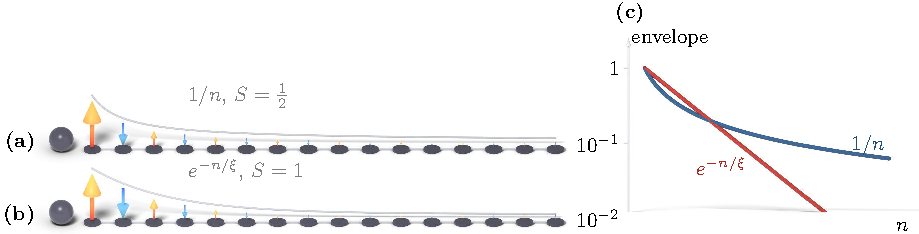
\includegraphics{figures/pdf/s09f05_decay.pdf}
\end{aqmfigure}
